%% 
%% Copyright 2019-2020 Elsevier Ltd
%% 
%% This file is part of the 'CAS Bundle'.
%% --------------------------------------
%% 
%% It may be distributed under the conditions of the LaTeX Project Public
%% License, either version 1.2 of this license or (at your option) any
%% later version.  The latest version of this license is in
%%    http://www.latex-project.org/lppl.txt
%% and version 1.2 or later is part of all distributions of LaTeX
%% version 1999/12/01 or later.
%% 
%% The list of all files belonging to the 'CAS Bundle' is
%% given in the file `manifest.txt'.
%% 
%% Template article for cas-sc documentclass for 
%% single column output.

%\documentclass[a4paper,fleqn,longmktitle]{cas-sc}
\documentclass[a4paper,fleqn]{cas-sc}

%\usepackage[numbers]{natbib}
%\usepackage[authoryear]{natbib}
\usepackage[authoryear,longnamesfirst]{natbib}

%%%Author macros
\def\tsc#1{\csdef{#1}{\textsc{\lowercase{#1}}\xspace}}
\tsc{WGM}
\tsc{QE}
\tsc{EP}
\tsc{PMS}
\tsc{BEC}
\tsc{DE}
%%%

\begin{document}

\title [mode = title]{Simulación de Nanotransportador de Titanio con Nanofibras Polimericas de liberación controlada para Vitiligo}                      




\author[1,3]{Denisse Leyva}[type=editor,
                        auid=,
                        prefix=,
                        role=,
                        orcid=0000-0001-7511-2910]
\cormark[1]
\fnmark[1]
\ead{cvr_1@tug.org.in}
\ead[url]{www.cvr.cc, cvr@sayahna.org}

\credit{Conceptualization of this study, Methodology, Software}

\address[1]{Facultad de Ingenieria Mecánica y Eléctrica}



\begin{abstract}
En el presente artículo se presenta una simulación para un nanotransportador de capa-coraza en el que buscamos una liberación de farmaco mas pronlongada, se propone que la liberación sea controlada con estimulos externos para que sea una liberación del fármaco mas eficiente y específica. Se abordarán tres estimulos externos y se podremos observar el analisis y eficiencia de cada uno.
\end{abstract}


\begin{keywords}
nanotransportador \sep nanofibras \sep Vitiligo \sep \BEC
\end{keywords}


\maketitle


\section{Introduction}
Las enfermedades de la piel son las cuartas afecciones cutáneas no mortales más importantes que actúan como una carga y afectan la economía mundial a nivel mundial. Esta condición afecta la calidad de vida del paciente y tiene un impacto pronunciado tanto en su estado físico como mental. El tratamiento de estas afecciones de la piel con enfoques convencionales muestra falta de eficacia, larga duración del tratamiento, recurrencia de afecciones, efectos secundarios sistémicos, etc., debido a la administración inadecuada del fármaco. Sin embargo, estos escollos pueden superarse con las aplicaciones de enfoques basados en nanomedicina que proporcionan una administración eficaz de fármacos en un sitio específico en el sitio objetivo. Estas estrategias basadas en nanomedicina evolucionan como posibles oportunidades de tratamiento en forma de nanoportadores, como nanoportadores poliméricos y lipídicos, nanoemulsiones y otros emergentes, nanotubos de carbono para tratamiento dermatológico. 

La liberación de medicamento de forma eficiente y localizada se ha convertido en uno de los retos mas importantes a resolver en nuestra sociedad actual. Se han evalúado numerosas alternativas en la aplicación de medicamento tales como la vía tópica, oftálmica, sublingual, transdermal, ótica, rectal y vaginal; teniendo distintos niveles de efectividad dependiendo del tipo de padecimiento a tratar. Pero todos ellos sin excepción adolecen de una falta de localización y programación en la aplicación del medicamento. Debido a lo anterior las mencionadas vías de administración de medicamento continúan provocando efectos secundarios que disminuyen la calidad de vida del paciente y lo llevan en situaciones extremas a abandonar el tratamiento prescrito por el médico. En este contexto, los científicos especializados en nanotecnología en conjunto con los profesionales de la salud han propuesto nuevos sistemas de liberación con la habilidad de transportar el medicamento a través del cuerpo y liberarlo de manera precisa y controlada en la zona afectada por un determinado padecimiento. Entre los sistemas nanoestructurados que se han utilizado en la administración controlada de medicamento se encuentran las nanopartículas, nanotubos, nanofibras y nanoesferas. Sin embargo, la tendencia mundial actual es elevar la sofisticación de estos materiales nanoestructurados en aras de incrementar su nivel de localización y programación en la liberación controlada de medicamentos.

En este sentido se han diseñado nanocompósitos que han combinado las propiedades deseadas de dos o mas nanoestructuras. Lo anterior con el objetivo de incrementar la habilidad de esos nanocompósitos para el transporte y liberación controlada y precisa de medicamento para el tratamiento de diversos padecimientos. Los resultados previos in vitro e in vivo de estos nanocompósitos ha sido también el incremento en la ‘programación’ de la liberación de medicamento; esto es, el medicamento no únicamente se libera de manera localizada sino que responde a una serie de estímulos fisiológicos que llevan a la interacción de estos nanocompósitos con el medio fisiológico circundante, algunas veces utilizando mecanismos biomiméticos tales como el autoensamblaje provocado por diferencias en pH o temperatura. Esta programación en la liberación de medicamento de igual manera se puede llevar a cabo en una serie de etapas para liberar no uno sino varias sustancias terapéuticas necesarias para atacar padecimientos multifactoriales tales como el cáncer o la artitris reumatoide. Esta liberación en etapas se ha convertido una característica deseada fundamental en los modernos sistemas de liberación de medicamento utilizando nanocompósitos, dado que aumenta las posibilidades de interacción del sistema de liberación con el medio ambiente fisiológico circundante, lo que aunado a la posibilidad de liberar mas de un tipo de medicamento, aumenta potencialmente la efectividad de los sistemas de liberación mas avanzados reportados en la literatura.

\section{Antecedentes}

Las nanofibras poliméricas son un tipo de nanoestructura 1D que tienen una relación area superficial contra volumen elevada, con diámetros que van de los 50 nm a los 500 nm en comparación con un largo reportado hasta los 1000 m1. Las nanofibras poliméricas tienen la particularidad de contar con una gran versatilidad de síntesis y de aplicaciones. Para producir las nanofibras poliméricas se han utilizado una variedad de técnicas incluyendo la separación de fases, el hilado por centrifuga, estiramiento, templete, autoensamblaje y el electrohilado (figura 1). De todas las técnicas mencionadas el electrohilado es por mucho la técnica mas utilizada en la fabricación de nanofibras poliméricas debido sobre todo a su sencillez y versatilidad.



Las nanofibras electrohiladas poliméricas han sido aprovechadas en la encapsulación y liberación de una variedad de medicamentos y sustancias terapéuticas a lo largo de la última década (tabla 1). Lo anterior debido a sus propiedades únicas de modulación de liberación a través de una variedad de morfologías obtenidas por medio de la modulación y control de los parámetros de solución y operación de la técnica de electrohilado. El diámetro de las NPE sintetizadas se debe de mantener lo mas delgado posible, esto debido a la relación reportada entre un diámetro pequeño de las nanofibras y una mayor rapidez en la liberación del medicamento. Otro factor a tomar en cuenta es la porosidad de los materiales nanofibrosos resultantes, dado que incide directamente en el perfil de liberación resultante.

Las nanofibras electrohiladas poliméricas se han utilizado en un amplio rango de aplicaciones tales como la filtración, sensado, aplicaciones electrónicas, catálisis, vendaje de heridas, ropa para protección química y biológica. Sin embargo es en el campo de la biotecnología donde las nanofibras electrohiladas poliméricas han encontrado sus aplicaciones más interesantes y relevantes desde el punto de vista científico, como la ingeniería de tejidos, órganos artificiales, la inmovilización de sustancias de interés biológico y la encapsulación y posterior liberación de medicamento y sustancias terapéuticas. Es en esta última aplicación biotecnológica de las NPE donde este proyecto propone ahondar mas en el estudio sistemático de las interacciones de las diferentes configuraciones y parámetros del sistema de electrohilado con la distribución de los medicamentos y sustancias terapéuticas a lo largo de los materiales nanofibrosos resultantes.


\begin{figure}[h]
	\centering
		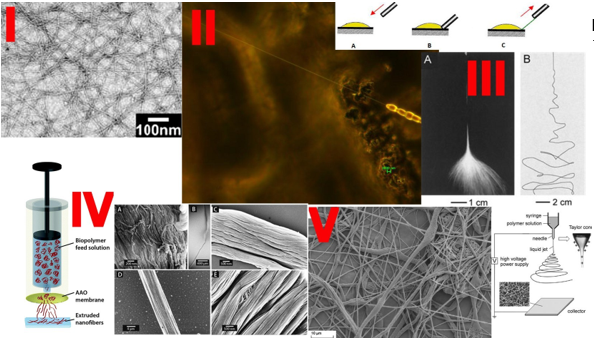
\includegraphics[scale=.75]{figs/Fig_1.png}
	\caption{Técnicas para producir nanofibras I)Autoensamblaje de peptidos, II)Estiramiento de una fibra de policrapolactona (PCL), III)Electrohilado de nanofibras polimericas, IV)Extrusión de nanofibras de un ensamblado de proteínas intracelulares, V)Fibras de PCL sintetizadas por el método de separación de fases.}
	\label{FIG:1}
\end{figure}

\section{Metodología}
Para esta simulación se tomaron en cuenta dos métodos diferentes (Sistema Multiagente e Interacciones entre partículas) que al utilizarse en conjunto nos acercan al objetivo deseado, se opto por esos métodos ya que el sistema multiagente representa el cambio de estado de las partículas y la interaccion entre partículas representa la acción que genera un choque de partículas.

\subsection{Sistema Multiagente}
El dominio del sistema multiagente o de inteligencia artificial distribuida es una ciencia y una técnica que trata con los sistemas de inteligencia artificial en red. El bloque fundamental de construcción de un sistema multiagente, como es de esperarse, son los agentes.

Aunque no existe una definición formal y precisa de lo que es un agente, estos son por lo general vistos como entidades inteligentes, equivalentes en términos computacionales a un proceso del sistema operativo, que existen dentro de cierto contexto o ambiente, y que se pueden comunicar a través de un mecanismo de comunicación ínter proceso, usualmente un sistema de red, utilizando protocolos de comunicación.

En cierto modo, un sistema multiagente es un sistema distribuido en el cual los nodos o elementos son sistemas de inteligencia artificial, o bien un sistema distribuido donde la conducta combinada de dichos elementos produce un resultado en conjunto inteligente.

\subsection{Interacción entre Partículas}
Dos partículas microscópicas, como las enzimas o los coloides, pueden tener una amplia gama de interacciones complejas, no se limitan solo a atraerse o repelerse, sino que cada partícula actúa como un espejo para su vecino, lo que origina nuevos patrones de comportamiento. Las partículas químicamente activas, como las enzimas o los coloides, pueden propulsarse en un líquido al convertir la energía química en trabajo mecánico. Una característica especial de estas partículas es que pueden violar la tercera ley de Newton: para un sistema de dos partículas, la acción y la reacción no son necesariamente iguales, ni siempre están en direcciones opuestas.
Sin embargo, a pesar de esta peculiaridad, la interacción relativa de estas partículas cuando están en su forma más simple posible, es decir, isotrópica y de igual tamaño, se suponía sencilla. Hasta ahora se pensaba que esta interacción era puramente atractiva (en cuyo caso las partículas se unen y forman un complejo), o puramente repulsiva (cuando las partículas se separan indefinidamente), como en cargas positivas y negativas en electrostática. Investigaciones recientes demuestran que la interacción entre dichas partículas a través de la señalización química y la modificación de su líquido circundante es en realidad mucho más compleja.
Según explican estas investigaciones, la relación entre dos partículas químicamente activas no siempre se puede clasificar como puramente atractiva o repulsiva. Por ejemplo, las partículas pueden moverse juntas como un estado unido estable, manteniendo una distancia de equilibrio constante entre ellas diferente de cero. En este caso, las partículas se repelen si se acercan más de una cierta distancia, y se atraen si se separan más.
Sin embargo, hay más posibilidades: las partículas también pueden hacer todo lo contrario.
Hay momentos en que las partículas, en vez de atraerse o repelerse, forman un inesperado complejo estable que puede romperse bajo suficientes perturbaciones o agitaciones.






\section{Criterios de Interacción}
Se escogieron tres estímulos para que el nanoportador libere el fármaco.

\begin{itemize}
  \item Temperatura
  \item PH
  \item Anticuerpos
\end{itemize}

Cuando el fármaco llegue a una temperatura diferente al ambiente el nanoportador entendera que es momento de liberar el fármaco sin afectar el ambiente externo a esa temperatura.


%\begin{table}[width=.9\linewidth,cols=4,pos=h]
%\caption{This is a test caption. This is a test caption. This is a test
%caption. This is a test caption.}\label{tbl1}
%\begin{tabular*}{\tblwidth}{@{} LLLL@{} }
%\toprule
%Col 1 & Col 2 & Col 3 & Col4\\
%\midrule
%12345 & 12345 & 123 & 12345 \\
%12345 & 12345 & 123 & 12345 \\
%12345 & 12345 & 123 & 12345 \\
%12345 & 12345 & 123 & 12345 \\
%12345 & 12345 & 123 & 12345 \\
%\bottomrule
%\end{tabular*}
%\end{table}

\section{Resultados y Discusión}




%% Loading bibliography style file
%\bibliographystyle{model1-num-names}
\bibliographystyle{cas-model2-names}

% Loading bibliography database
\bibliography{cas-refs}


%\vskip3pt

\end{document}

